\documentclass[11pt,a4paper,english]{article}
\usepackage[utf8]{inputenc}
\usepackage[shortlabels]{enumitem}
\usepackage[margin=0.85 in]{geometry}
\usepackage{datetime}
\usepackage{parskip}
\usepackage{graphicx}
\usepackage{hyperref}
\usepackage{fancyhdr}
\pagestyle{fancy}
%\usepackage{fourier-orns}  %The special head rule
%\renewcommand\headrule{\hrulefill
%\raisebox{-2.1pt}[10pt][10pt]{\quad\decofourleft\decotwo\decofourright\quad}\hrulefill}

\setlength{\parskip}{1em}
\usepackage{titlesec}

\titlespacing{\section}{0pt}{10pt plus 4pt minus 2pt}{0pt plus 2pt minus 2pt}
\titlespacing{\subsection}{0pt}{10pt plus 4pt minus 2pt}{-2pt plus 2pt minus 2pt}
% the above adjust the heading spacing, {}{left margin}{top margin}{after-sep} 10pt plus 4pt (can stretch up to 4pt, 2pt, shrink to 2pt

\usepackage{titling}
\setlength{\droptitle}{-4em}


\lhead{\textsl{Qianyue Zhang}}
\rhead{\textsl{Downing College}}

\usepackage{csquotes} % Recommended for natbib package...
\usepackage{natbib}
\renewcommand*{\bibfont}{\raggedright}
\renewcommand*{\bibfont}{\tiny}

\title{\textbf{Dynamic Simulation, Optimisation and Control of Biochemical Processes—Three-Month Report}}
\author{\textbf{Qianyue Zhang}\\
Downing College\\
Supervisor: Dr Vassilios S. Vassiliadis\\
Advisor: Dr Ljiljana Fruk}
\longdate


\begin{document}
\maketitle
\thispagestyle{fancy}
\section*{Summary}
This PhD project is focused on \textit{in silico} simulation to model, predict, optimise and control dynamic biochemical processes. While this report outlines a detailed framework with a planned timeline and objectives to achieve its first milestone—setting out to improve and extend the methodology proposed by \citet{scott2018simulation}, using an Interior Point Method (IPM) to simulate and optimise Dynamic Flux Balance Analysis (dFBA) models. Thereafter, it will continue the dFBA topics and potentially be extended to include research on cell signalling simulation.
\section*{Introduction}
Microbial systems have a huge potential in producing high value bioproducts (\textit{e.g.} nutrition supplements and pharmaceuticals). Yet they are far from being accurately modelled and analysed, nor can they controlled as precisely as other standard chemical engineering reaction systems.  Tackling this problem will lead to significant improvement in the efficiency of the biochemical processes.

The first challenge facing many scientists and engineers is that there is a multitude of complicated kinetics taking place within a living cell, in different compartments, for example, in mitochondria in eukaryotic cells for energy generation, and in ribosomes for protein generation. To simulate all these reactions within a cell is very difficult as kinetics for them cannot be readily estimated. Therefore, Flux Balance Analysis (FBA) is introduced, which is a stochiometric modelling approach that represents mathematically the biochemical networks that range from small-scale to genome-scale metabolic reconstructions within a cell, assuming quasi-steady state. FBA works by constructing only the steady state metabolite material balance within the cell, based on the stoichiometry of the reaction involved only. Coupling with extracellular conditions by suitable uptake and secretion rate functions, \textit{e.g.} Monod kinetic, a Linear Programming (LP) problem can be constructed to optimise a sole objective—“goal of the microorganisms”—typically it is something that reflex their survival, \textit{e.g.} by maximising biomass or energy reserve (ATP) rates.

FBA assumes microbial cells are immersed in an extracellular environment that is constant and not influencing the intracellular environment. In real life, however, cells are cultivated in either batch or fed-batch processes, where surrounding nutrient levels vary with time. Therefore, dFBA, an extension of FBA, adds the dynamic variation of the metabolites in the modelling formalism of FBA, improving the prediction of the behaviour cultures of microorganism, such that it can match better experimental results and industrial operation. While it assumes intracellular quasi-steady state, this has proven to be a mild assumption which does not detract from the predictive ability of the methodology. The dFBA model is in effect a LP model being embedded within a set of dynamic material balances for the extracellular environment, which are modelled typically as Ordinary Differential Equations (ODEs).

There are several dFBA simulation tools and methods that have been proposed, including the static optimisation approach, the dynamic optimisation approach, the direct approach and DFBAlab \citep{harwood2016efficient}, though they each has different advantages and disadvantages as simulation tools. \citep{scott2018simulation} sought to introduce another highly competitive simulation method for dFBA, based on an IPM which can solve large-scale dFBA problem accurately and quickly, and is able to be used to control the bio-cultures involved \citep{Vassiliadis2018,monteiro1989interior}.  Presenting in detail this new approach would be too demanding for this short report, but in essence the new idea presented is to transform the embedded LP problem within the dFBA model involving advanced optimisation techniques, namely the use of IPM to transform the LP into a set of algebraic equations (full details can be found again in \citep{scott2018simulation}).

Another challenge that limits the accurate modelling and simulation of biochemical production process is that microbial communities usually coexist and interact through the common culture medium, often lead to influencing each other’s kinetics. It is reported that the synergistic combination of different species can lead to potential advantages in resource utilisation in many cases \citep{henson2014dynamic,gomez2016sugars}. Therefore, this project will take co-culture simulation into consideration so as the result of the project can potentially be used as an industry guide on the optimisation and control of realistically complex microbial cultures.

The overall methodology for this project is shown as a flowchart in \textbf{Figure \ref{fig:my_label}}. There are three main objectives which must be met to achieve this overall aim:
\begin{enumerate} [(A)]
    \item Construct dFBA models of a single microbial species.
    \item Optimise, predict and validate the performance of the model.
    \item In-depth simulation of co-culture model.
\end{enumerate}
\begin{figure}[ht]
    \centering
    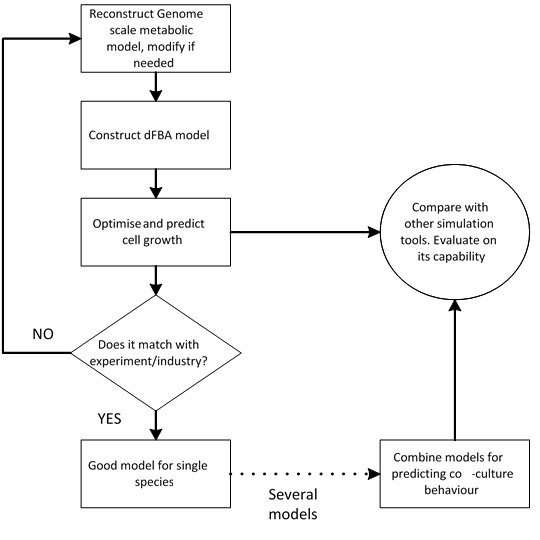
\includegraphics[width=12cm]{projectmethodology.png}
    \caption{The simplified project methodology with key steps}
    \label{fig:my_label}
\end{figure}

\section*{Project Methodology}
\subsection*{\underline{(A) Construct dFBA model of a single microbial species}}
\label{sec:subsecA}
To construct the models, Mr. Prakitr Srisuma’s work can act as a starting point\citep{Srisuma2018}. This step can be achieved by reproducing and subsequently improving on the models presented in that work. This step can be done rather quickly since the Matlab code is provided. However, the code might have some errors, and time would be required to rectify these. Three weeks from now should be enough to get it to run. Following that, several new issues have to be addressed at this phase of the project:

\begin{enumerate}
\item
The sources of the data need to be selected carefully in order to match with experiment.
\item
The objectives and constraints in the case study can be changed to more realistic ones, for example to maximise the total growth rate \citep{henson2014dynamic}.
\end{enumerate}

\subsection*{\underline{(B) Optimise, predict and validate the performance of the model}}
\label{sec:subsecB}
The model generated in item \hyperref[sec:subsecA]{(A)} should be validated with experimental data. This step is crucial and by the IPM approach for dFBA to be shown that it can accurately simulate experimental processes, its reliability will be strengthened. Further work can be carried out to test the range of inputs and operating conditions for which the model is reliable so that its flexibility is also validated.

\subsection*{\underline{(C) In-depth simulation of co-culture model}}
\label{sec:subsecC}
As mentioned above, this project focuses on the capability of the IPM approach for dFBA in modelling large-scale, co-culture metabolic systems. It is proposed to examine the interaction between \textit{Saccharomyces Cerevisiae} and \textit{Komagataella Phaffii}. The interesting point about these two yeasts is that the former can produce ethanol in anaerobic fermentation which inhibits the growth of the latter, while the latter can consume methanol \citep{tuttle1995divergent}. The successful prediction of this co-culture model can be used to explore further the advantages of the IPM approach for dFBA. By the end of the first year, it is aimed to have explored the following items:
\begin{enumerate}
    \item 
The application of the model and capability of the IPM approach for dFBA in the simulation of dynamic microbial co-culture systems.
    \item
Explore whether the stoichiometric matrix in the dFBA model can be constructed in a way to include the interactions of the co-culture, so as to consider a co-culture system as a new, integrated system.
    \item
    Use dynamic optimisation for parameter fitting of kinetic models integrated within the dFBA model, so as to accurately model such dynamic systems.
    \item
Explore the dynamics of the population of microbial system described by \citet{lee2009individual} to account for different phenotypes arise from difference in the molecular level.
\end{enumerate}
The successful completion of the tasks in the above itemised list can lead to publishable papers, which is one of the aims during the first year of this project. Moreover, this project can be extended to include nonlinear convex objective functions for the FBA embedded problem with the dFBA model so as to further expand the capability of this powerful simulation approach—a nonlinear objective function may be able to capture better the objective/operation of the intracellular biochemical reaction networks considered for different microorganisms.

The projected timeline for the first year of research and studies on this project is illustrated in the Gantt chat shown below in \textbf{Figure \ref{fig:my_label2}}.

\begin{figure}[ht]
    \centering
    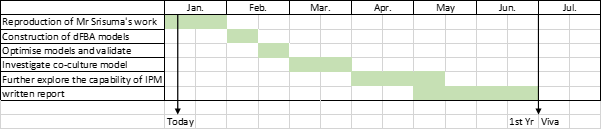
\includegraphics[width=\textwidth]{Gantt.png}
    \caption{Detailed timeline for the first year of research}
    \label{fig:my_label2}
\end{figure}

The first two items—the \hyperref[sec:subsecA]{(A)} \& \hyperref[sec:subsecB]{(B)} project methodologies listed above—can be achieved relatively easily, but a solid and reliable model created in these items is crucial in the following steps. Approaching March, it is planned to start working on co-culture systems. The entry “Further explore the capability of IPM” includes the investigation of microbial ecosystem of several, instead of two, communities; the stochastic modelling approach of differentiated cell groups and the simulation of non-convex objectives.

\section*{Current Progress} 
Intensive literature review of the dFBA approach and the IPM was carried out in the past three months during commencement of this project, alongside with a thorough understanding of the representation of genome-scale metabolic networks. Furthermore, Mr.Srisuma’s Matlab code was thoroughly studied with some mistakes identified already and under correction currently—with this particular task not completed as yet. 

\section*{Conclusions}
The introduction states a defined overall methodology that sets a pathway to reach the aim of this project. The detailed project methodology provides a clear step-by-step outline of what should be taken in the next nine months and so to achieve the first milestone. The ambitious first year goal is to assess the IPM approach for dFBA and to obtain publishable results.  

\bibliographystyle{agsm} % Havard set of Bibliography Style--round, author-year
\bibliography{Ref}


\end{document}









